\documentclass[a4paper,12pt]{article}

%%% Работа с русским языком
\usepackage{cmap}					% поиск в PDF
\usepackage{mathtext} 				% русские буквы в формулах
\usepackage[T2A]{fontenc}			% кодировка
\usepackage[utf8]{inputenc}			% кодировка исходного текста
\usepackage[english,russian]{babel}	% локализация и переносы
\usepackage{indentfirst}            % красная строка в первом абзаце
\usepackage{extarrows}              % длинное равно
\frenchspacing                      % равные пробелы между словами и предложениями

%%% Дополнительная работа с математикой
\usepackage{amsmath,amsfonts,amssymb,amsthm,mathtools} % пакеты AMS
\usepackage{icomma}                                    % "Умная" запятая
\usepackage{physics} % для символа нормы

%%% Свои символы и команды
\usepackage{centernot} % центрированное зачеркивание символа
\usepackage{stmaryrd}  % некоторые спецсимволы

\usepackage{pythonhighlight}

% \renewcommand{\epsilon}{\ensuremath{\varepsilon}}
% \renewcommand{\phi}{\ensuremath{\varphi}}
% \renewcommand{\kappa}{\ensuremath{\varkappa}}
% \renewcommand{\le}{\ensuremath{\leqslant}}
% \renewcommand{\leq}{\ensuremath{\leqslant}}
% \renewcommand{\ge}{\ensuremath{\geqslant}}
% \renewcommand{\geq}{\ensuremath{\geqslant}}
% \renewcommand{\emptyset}{\ensuremath{\varnothing}}

% \DeclareMathOperator*{\Mid}{\scalebox{1.1}{$\mid$}}
\DeclareMathOperator*{\argmax}{argmax}

% \DeclareMathOperator{\sgn}{sgn}
% \DeclareMathOperator{\gd}{\text{НОД}}
% \DeclareMathOperator{\lf}{\text{НОК}}
% \DeclareMathOperator{\rk}{rk}
% \DeclareMathOperator{\pr}{pr}
% \DeclareMathOperator{\im}{Im}
% \DeclareMathOperator{\ke}{Ker}
% \DeclareMathOperator{\re}{Re}
% \DeclareMathOperator{\cha}{char}
% \DeclareMathOperator{\ord}{ord}
% \DeclareMathOperator{\tr}{tr}
% \DeclareMathOperator{\md}{mod}
% \DeclareMathOperator{\Aut}{Aut}
% \DeclareMathOperator{\Inn}{Inn}
% \DeclareMathOperator{\End}{End}
% \DeclareMathOperator{\GL}{GL}
% \DeclareMathOperator{\SL}{SL}
% \DeclareMathOperator{\diag}{diag}

\newcommand{\divby}{
	\mathrel{\vbox{\baselineskip.65ex\lineskiplimit0pt\hbox{.}\hbox{.}\hbox{.}}}
}
\newcommand{\notdivby}{\centernot\divby}
% \newcommand\norm[1]{\left\lVert#1\right\rVert}
% \newcommand\normx[1]{\left\Vert#1\right\Vert}
\newcommand{\N}{\mathbb{N}}
\newcommand{\Z}{\mathbb{Z}}
\newcommand{\Q}{\mathbb{Q}}
\newcommand{\R}{\mathbb{R}}
\newcommand{\E}{\mathbb{E}}
\newcommand{\D}{\mathbb{D}}
\newcommand{\Cm}{\mathbb{C}}
\newcommand{\F}{\mathbb{F}}
\newcommand{\id}{\mathrm{id}}
\newcommand{\imp}[2]{(#1\,\,$\ra$\,\,#2)\,\,}
\newcommand{\nset}[1]{\{1, \dotsc, #1\}}
\newcommand{\Chi}{\scalebox{1.1}{\raisebox{\depth}{$\chi$}}}
\newcommand{\FF}{\scalebox{0.95}{$\mathcal F$}}
\newcommand{\FFF}{\scalebox{0.55}{$\mathcal F$}}
\newcommand{\GG}{\scalebox{0.95}{$\mathcal G$}}
\newcommand{\GGG}{\scalebox{0.55}{$\mathcal G$}}

\newcommand{\ND}[2]{\mathcal{N}\left({#1}, {#2}\right)} % normal distribution
\newcommand{\tod}{\xrightarrow[]{d}}
\newcommand{\toP}{\xrightarrow[]{P}}
\newcommand{\tolp}[1]{\xrightarrow[]{L_{#1}}}
\newcommand{\toac}{\xrightarrow[]{\text{п. н.}}} % almost certainly

\renewcommand\labelitemi{$\triangleright$}
\newcommand{\LL}{\mathcal{L}}
\newcommand{\todo}[1]{\textcolor{red}{TODO} #1}
\let\bs\backslash
\let\vect\overline
\let\normal\trianglelefteqslant
\let\lra\Leftrightarrow
\let\ra\Rightarrow
\let\la\Leftarrow
\let\gl\langle
\let\gr\rangle
\let\sd\leftthreetimes
\let\emb\hookrightarrow
\let\mc\mathcal
\let\mf\mathfrak

%%% Перенос знаков в формулах (по Львовскому)
\newcommand*{\hm}[1]{#1\nobreak\discretionary{}{\hbox{$\mathsurround=0pt #1$}}{}}
\renewcommand{\phi}{\varphi}
\newcommand{\eps}{\varepsilon}

%%% Работа с картинками
\usepackage{graphicx}    % Для вставки рисунков
\setlength\fboxsep{3pt}  % Отступ рамки \fbox{} от рисунка
\setlength\fboxrule{1pt} % Толщина линий рамки \fbox{}
\usepackage{wrapfig}     % Обтекание рисунков текстом

%%% Работа с таблицами
\usepackage{array,tabularx,tabulary,booktabs} % Дополнительная работа с таблицами
\usepackage{longtable}                        % Длинные таблицы
\usepackage{multirow}                         % Слияние строк в таблице

%%% Теоремы
\theoremstyle{definition}
\newtheorem{problem}{}
\newtheorem{theorem}{Теорема}
\newtheorem*{lemma}{Лемма}
% \newtheorem{proposition}{Утверждение}[section]
% \newtheorem*{exercise}{Упражнение}
% \newtheorem{problem}{}

% \theoremstyle{definition}
% \newtheorem{definition}{Определение}[section]
% \newtheorem*{corollary}{Следствие}
% \newtheorem*{note}{Замечание}
% \newtheorem*{reminder}{Напоминание}
% \newtheorem*{example}{Пример}

\theoremstyle{remark}
\newtheorem*{solution}{Решение}
\newtheorem*{guidance}{Указание}
\newtheorem*{prooff}{Д-во}

%%% Оформление страницы
\usepackage{extsizes}     % Возможность сделать 14-й шрифт
\usepackage{geometry}     % Простой способ задавать поля
\usepackage{setspace}     % Интерлиньяж
\usepackage{enumitem}     % Настройка окружений itemize и enumerate
\setlist{leftmargin=25pt} % Отступы в itemize и enumerate

\geometry{top=25mm}    % Поля сверху страницы
\geometry{bottom=30mm} % Поля снизу страницы
\geometry{left=20mm}   % Поля слева страницы
\geometry{right=20mm}  % Поля справа страницы

\setlength\parindent{15pt}                % Устанавливает длину красной строки 15pt
\linespread{1.3}                          % Коэффициент межстрочного интервала
%\setlength{\abovedisplayskip}{3pt}       % Отступы от выключных формул
%\setlength{\belowdisplayskip}{3pt}       % Отступы от выключных формул
%\setlength{\abovedisplayshortskip}{3pt}  % Отступы от выключных формул
%\setlength{\abovedisplayshortskip}{3pt}  % Отступы от выключных формул
%\setlength{\parskip}{0.5em}              % Вертикальный интервал между абзацами
%\setcounter{secnumdepth}{0}              % Отключение нумерации разделов
%\setcounter{section}{-1}                 % Нумерация секций с нуля
\usepackage{multicol}			          % Для текста в нескольких колонках
\usepackage{soulutf8}                     % Модификаторы начертания

%%% Содержаниие
\usepackage{tocloft}
\renewcommand{\thesection}{\arabic{section}.} 
\renewcommand{\thesubsection}{\thesection.\arabic{subsection}.}
\tocloftpagestyle{main}
%\setlength{\cftsecnumwidth}{2.3em}
%\renewcommand{\cftsecdotsep}{1}
%\renewcommand{\cftsecpresnum}{\hfill}
%\renewcommand{\cftsecaftersnum}{\quad}

%%% Шаблонная информация для титульного листа
\newcommand{\CourseName}{Математическая статистика}
\newcommand{\FullCourseName}{\so{МАТЕМАТИЧЕСКАЯ СТАТИСТИКА}}
\newcommand{\TaskNumber}{II}
\newcommand{\CourseDate}{весна 2024}
\newcommand{\AuthorInitials}{Яфаров Руслан}

%%% Колонтитулы
% \usepackage{titleps}
% \newpagestyle{main}{
% 	\setheadrule{0.4pt}
% 	\sethead{\CourseName}{}{\hyperlink{intro}{\;Назад к содержанию}}
% 	\setfootrule{0.4pt}                       
% 	\setfoot{ФПМИ МФТИ, \CourseDate}{}{\thepage} 
% }
% \pagestyle{main}  

%%% Нумерация уравнений
\makeatletter
\def\eqref{\@ifstar\@eqref\@@eqref}
\def\@eqref#1{\textup{\tagform@{\ref*{#1}}}}
\def\@@eqref#1{\textup{\tagform@{\ref{#1}}}}
\makeatother                      % \eqref* без гиперссылки
\numberwithin{equation}{section}  % Нумерация вида (номер_секции).(номер_уравнения)
\mathtoolsset{showonlyrefs=false} % Номера только у формул с \eqref{} в тексте.

%%% Гиперссылки
\usepackage{hyperref}
% \usepackage[usenames,dvipsnames,svgnames,table,rgb]{xcolor}
\hypersetup{
	unicode=true,            % русские буквы в раздела PDF
	colorlinks=true,       	 % Цветные ссылки вместо ссылок в рамках
	linkcolor=black!15!blue, % Внутренние ссылки
	citecolor=green,         % Ссылки на библиографию
	filecolor=magenta,       % Ссылки на файлы
	urlcolor=NavyBlue,       % Ссылки на URL
}

%%% Графика
\usepackage{tikz}        % Графический пакет tikz
\usepackage{tikz-cd}     % Коммутативные диаграммы
\usepackage{tkz-euclide} % Геометрия
\usepackage{stackengine} % Многострочные тексты в картинках

\begin{document}
	\begin{titlepage}
	\clearpage\thispagestyle{empty}
	\centering
	
	\textbf{Московский физико-технический институт}
	\vspace{33ex}
	
	{\textbf{\FullCourseName}}
	
	\TaskNumber\ ЗАДАНИЕ 
	\vspace{1ex}

	\begin{flushright}
		\noindent
		Автор: {\AuthorInitials},
		\\
		Б13-202 
	\end{flushright}
	
	\vfill
	\CourseDate
	\pagebreak
\end{titlepage}
	\section{Элементы комбинаторики}
	\problem{Имеются $m$ белых и $n$ чёрных шаров, причём $m > n$. Сколькими способами можно разложить все шары в ряд так, чтобы никакие два чёрных
шара не лежали рядом?}
    \solution{Расставим все чёрные шары. Для белых шаров останется $m + 1$ место, куда можно положить шар. Тогда ответ - $C_{m+1}^n$}
    \problem{Сколько различных пар можно образовать из 28 костей домино так,
чтобы кости, входящие в пару, можно было приложить друг к другу?}
    \solution{Сначала рассмотрим вариант, когда одна из доминошек - дубль. Вторую доминошку определяет одно число не равное числу на первой доминошке. Дублей 7, чисел, не равных первому 6 $\Rightarrow$ вариантов $6 * 7 = 42$. Пусть теперь среди доминошек нет дублей. Выберем число, по которому соприкасаются доминошки. Остаётся выбрать пару $(a, b)$ так, что $a < b$ (ведь доминошки разные) и $a, b \ne$ выбранному числу. Тогда таких вариантов $7 * (1 + 2 + 3 + 4 + 5) = 105$ \\ Ответ: 147}
    \problem{Сколькими способами 12 полтинников можно разложить по пяти различным пакетам, если ни один из пакетов не должен быть пустым?}
    \solution{Положим в каждый пакет по полтиннику. Останется неупорядоченная выборка из 7 элементов по 5, т. е. ответ - $C_{5 + 7 - 1}^{7}$.
    \\ Ответ: $C_{11}^{7}$}
    \problem{~
    \begin{enumerate}[label=\alph*]
        \item Доказать, что число всевозможных подмножеств конечного множества, содержащего $n$ элементов, равно $2^n$.
       \item В множестве из n элементов выбираются подмножества $A$ и $B$ так, что $A \subset B$ и $A \neq B$. Доказать, что количество таких пар $(A, B)$ равно $3^n - 2^n$.
    \end{enumerate}
    }
    \solution{~
    	\begin{enumerate}[label=\alph*]
            \item Пусть $A = \{a_1, a_2, \cdots, a_n\}$. Поставим каждому $B \subset A$ в соответсвие двоичное число из n бит, на i бите 1, если $a_i \in B$ и 0 иначе. Очевидно, что соответсвие взаимно однозначно. Всего n-битных чисел $2^n$.
            \item Пар $(A, B)$ : $|B| = k, A \subseteq B \ 2^k C_n^k$. Тогда всего пар $\sum_{k = 0}^n 2^k C_n^k = (1 + 2)^n$. Пар вида $(A, A)\ 2^n \Rightarrow$ Ответ $3^n - 2^n$.  
        \end{enumerate}

    }
    \problem{Доказать, что множество из n элементов можно разбить $\frac{n!}{m_1!m_2!\cdots m_k!}$
различными способами на k попарно непересекающихся подмножеств,
содержащих по $m_1 , m_2 , \cdots , m_k$ элементов, где $m_1 + m_2 + \cdots + m_k$ = n
и числа $m_1 , m_2 , \cdots , m_k$ попарно различны.}
    \solution{Представим себе, что порядок в каждом из k множеств важен. Тогда кол-во способов разбить все элементы $n!$ (рассматриваем перстановки элементов, первые $m_1$ - в первое множество, следующие $m_2$ во второе и т. д.). Теперь предположим, что порядок в первом множестве неважен. Тогда предыдущий ответ в $m_1!$ больше настоящего $\Rightarrow$ настоящий $\frac{n!}{m_1!}$. Также для второго и т. д. получим $\frac{n!}{m_1!m_2!\cdots m_k!}$.}
    \problem{Сколькими различными способами можно разбить множество из 10 элементов на два подмножества из 3 элементов и два подмножества из 2 элементов?}
    \solution{Аналогично логике предыдущей задаче получим ответ $\frac{10!}{3!3!2!2!}$, но подмножества по 3 элемента неотличимы, так же как и по 2 $\Rightarrow$ Ответ $\frac{10!}{3!3!2!2!2!2!}$}
    \problem{Для пилки дров выделено 14 человек. Сколькими способами их можно разделить на пары?}
    \solution{Аналогично предыдущей задаче $\frac{14!}{7!(2!)^7}$}
    \problem{Сколькими способами можно выбрать из полной колоды, содержащей 52 карты, 6 карт так, чтобы среди них были все четыре масти? (В полной колоде имеется по 13 карт каждой масти.)}
    \solution{
    Возможны 2 интересующих нас варианта: либо в колоде 3 карты одной масти, а остальные карты разл. масти, либо 2 карты одной масти, 2 другой, а остальные разл. Тогда ответ $C_4^1C_9^3(C_9^1)^3 + C_4^2(C_9^2)^2(C_9^1)^2$ 
    }
    \problem{
    	Найти номер наибольшего члена в разложении $(a + b)^n$, если:
    	\begin{enumerate}[label=\alph*]
    		\item $a = \frac{2}{3}, b = \frac{1}{3}, n = 100$;
    		\item $a = b = \frac{1}{2}, n = 100$;
    		\item $a = b = \frac{1}{2}, n = 99$.
    	\end{enumerate}
    }
    \solution{~
    	\begin{enumerate}[label=\alph*]
    		\item $\left(\frac{2}{3} + \frac{1}{3}\right)^{100} = \sum_{k = 0}^n \frac{2^k}{3^k}\frac{1}{3^{n - k}}\frac{100!}{k!(100-k)!} =
    		\frac{100!}{3^n}\sum_{k = 0}^n \frac{2^k}{k!(100 - k)!}\text{. Положим } a_k = \frac{2^k}{k!(100 - k)!}$\\
    		$\text{Тогда } k_{\text{иск}} = \argmax_{0 \le k \le 100} a_k. \ \frac{a_k}{a_{k - 1}} = \frac{2(101 - k)}{k} > 1 \text{ при } k < \frac{202}{3} \Rightarrow k_{\text{иск}} = 67$;
    		\item Аналогично a. $a_k = \frac{1}{k!(100 - k)!}$. $\frac{a_k}{a_{k - 1}} = \frac{101 - k}{k} > 1 \Rightarrow k < \frac{101}{2} \Rightarrow k_{\text{иск}} = 50$;
    		\item Аналогично a. $a_k = \frac{1}{k!(99 - k)!}$. $\frac{a_k}{a_{k - 1}} = \frac{100 - k}{k} > 1 \Rightarrow k < 50 \Rightarrow k_{\text{иск}} = 49$.
    	\end{enumerate}
    }
    \problem{
    	Доказать тождества:
    	\begin{enumerate}[label=\alph*]
    		\item $C_n^k = C_n^{n - k}$, если $0 \le k \le n$;
    		\item $C_{n + 1}^{k + 1} = C_n^k + C_n^{k + 1}$, если $0 \le k \le n - 1$;
    		\item $\sum_{k = 0}^n C_n^k = 2^n$;
    		\item $\sum_{k = 0}^n (C_n^k)^2 = C_{2n}^n$;
    		\item $C_n^n + C_{n + 1}^n + \cdots C_{n + m - 1}^n = C_{n + m}^{n + 1}$, если $m \ge 1$.
    	\end{enumerate}
    }
    \solution{
    	\begin{enumerate}[label=\alph*]
    		\item $C_n^k$ показывает кол-во неупорядоченных выборок из k элементов по n без возвращений, но когда мы выбираем k элементов, мы оставляем $n - k$ элементов, которую можно рассматривать как выборку из $n - k$ элементов без возвращений. $\Rightarrow C_n^k = C_n^{n - k}$;
    		\item Покрасим один из элементов множетсва. Тогда кол-во способов выбрать $k + 1$ элементов из множества мощности n равно кол-во способов выбрать $k$ элементов из множества без закрашенного элемента(мы его уже взяли) + кол-во способов выбрать $k + 1$ элемент из множества без закрашенного элемента(мы его не берем) $\Rightarrow C_{n + 1}^{k + 1} = C_n^k + C_n^{k + 1}$, если $0 \le k \le n - 1$;
    		\item Решим задачу 4a иначе. Сначала посчитаем сколько есть подмножеств $A$ мощности 0 - $C_n^0$. Затем можности 1 - $C_n^1$. $\cdots$ мощности $k$ - $C_n^k$ Получим, что $\sum_{k = 0}^n C_n^k = 2^n$;
    		\item $C_{2n}^n$ Показывает кол-во подмножеств мощности $n$ множества мощности $2n$. Положим $A_1 = \{a_1, a_2, \cdots, a_n\}$, $A_2 = \{a_{n + 1}, a_{n + 2}, \cdots, a_{2n}\}$ Тогда $n$ элементов можно выбрать $n + 1$ способом - 0 из $A_1$, $n$ из $A_2$, 1 из $A_1$, $n - 1$ из $A_2$ и т.д. $C_{2n}^n = \sum_{k = 0}^n C_n^kC_n^{n - k} = \sum_{k = 0}^n (C_n^k)^2$;
    		\item Крч комбинаторно я не смог, по индукции изи(.
    	\end{enumerate}

    }
    \problem{Доказать, что сумма чисел $C_n^k$ по всем чётным $k$ равна сумме чисел $C_n^k$ по всем нечётным $k$.}
    \solution{abc}
    \section{Вероятностное пространство $(\Omega, \mathcal{A}, P)$}
    \problem{Из урны, содержащей $M$ различных шаров, наудачу последовательно
извлекаются $n$ шаров. Рассмотреть два способа выбора: с возвращением
и без возвращения; описать для каждого способа структуру простран-
ства элементарных событий и подсчитать число элементов в  в случае
упорядоченных и неупорядоченных выборок.}
	\solution{~
	\begin{itemize}
		\item Без возвращения упорядоченно. $\Omega = \{(a_1, a_2, \cdots, a_n) | 1 \le a_i \le M, a_i \ne a_j \text{ при } i \ne j\}$
		$|\Omega| = A_M^n$
		\item Без возвращения неупорядоченно. $\Omega = \{\{a_1, a_2, \cdots, a_n\} | 1 \le a_i \le M, a_i \ne a_j \text{ при } i \ne j\}$
		$|\Omega| = C_M^n$
		\item С возвращением упорядоченно. $\Omega = \{(a_1, a_2, \cdots, a_n) | 1 \le a_i \le M\}$
		$|\Omega| = M^n$
		\item С возвращением неупорядоченно. $\Omega = \{\{a_1, a_2, \cdots, a_n\} | 1 \le a_i \le M\}$
		$|\Omega| = C_{M + n - 1}^n$
	\end{itemize}
	Во всех случаях $\mathcal{A} = 2^{\Omega}$
	}
	\problem{Пусть $A$ и $B$ произвольные события. Проверить справедливость следующих соотношений:
\[ \overline{(\overline{A})} = A; A \setminus B = A \setminus AB = A\overline{B}; A \setminus (A \setminus B) = AB; \]
\[ A \subseteq B \Rightarrow \overline{B} \subseteq \overline{A}; \overline{A \cup B} = \overline{A} \cap \overline{B}; \overline{A \cap B} = \overline{A} \cup \overline{B}; \]
\[ (A \cup B) \cap C = (A \cap B) \cup (B \cap C) \]
\[ (A \cap B) \cup C = (A \cup B) \cap (B \cup C) \]
}
	\solution{~
	\begin{enumerate}
		\item $\overline{(\overline{A})} = \Omega \setminus \overline{A} = \Omega \setminus (\Omega \setminus A) = A$
		\item
		\[x \in A \setminus AB \Leftrightarrow x \in A \land x \notin AB \Leftrightarrow x \in A \land (x \notin A \lor x \notin B) \Leftrightarrow x \in A \land x \notin B \Leftrightarrow x \in A \setminus B\]
		\[\Leftrightarrow x \in A \land x \notin B \Leftrightarrow x \in A \land x \in \overline{B} \]
		\item Пользуясь 2. и 1. 
		\[ A \setminus (A \setminus B) = A \setminus A\overline{B} = A\overline{\overline{B}} = AB \]
		\item $x \in \overline{B} \Rightarrow x \notin A (\text{иначе бы } x \in B) \Rightarrow x \in \overline{A}$
		\item $x \notin (A \cup B) \Leftrightarrow x \notin A \land x \notin B \Leftrightarrow x \in \overline{A} \cap \overline{B}$
		\item $x \notin (A \cap B) \Leftrightarrow x \notin A \lor x \notin B \Leftrightarrow x \in \overline{A} \cup \overline{B}$
		\item
		\[ x \in (A \cup B) \cap C \lra x \in (A \cup B) \land x \in C \lra x \in A \cap C \lor x \in B \cap C \lra x \in (A \cap C) \cup (B \cap C)\]
		\item
		\[ x \in (A \cap B) \cup C \lra x \in (A \cap B) \lor x \in C \lra x \in A \cup C \land x \in B \cup C \lra x \in (A \cup C) \cap (B \cup C)\]
	\end{enumerate}
	}
	\problem{Пусть $A_n = [a, a + \frac{1}{n}), B_n = [a, b - \frac{1}{n}]$, где $n = 1, 2, \cdots, \ a$ и $b$ - действительные числа. Найти $\cap_{n = 1}^{\infty}A_n$ и $\cup_{n = 1}^{\infty}B_n$}
	\solution{
	Пусть $A = \cap_{n = 1}^{\infty}A_n$, $B = \cup_{n = 1}^{\infty}B_n$
	Предположим $\exists c \in A : c > a$. Тогда $c \in \cap_{n = 1}^{N}A_n$, где $N = \lceil \frac{1}{c - a}\rceil$, но $c \notin A_N$. Очевидно $a \in A \ra A = \{a\}$. Аналогично доказывается, что $B = [a, b]$  
	}
	\problem{Электрическая цепь между точками $M$ и $N$ составлена по схеме, при-
ведённой на рисунке.
	\begin{center}
	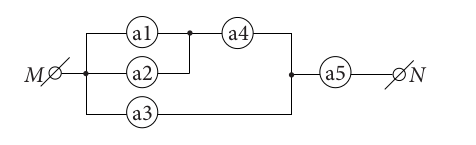
\includegraphics[scale=0.8]{pictures/chain.png}
	\end{center}
	Выход из строя элемента $a_i$ событие $A_i$ ($i = 1, \cdots, 5$). Записать выражения для событий $\overline{C}$ и $C$ , если $C$ означает разрыв в цепи.
}
	\solution{
	    $\overline{C} = \{\{A_3, A_1\}, \{A_3, A_2\}, \{A_4, A_1\}, \{A_4, A_2\}, \{A_4, A_2, A_1\}, \{A_1, A_2\}, \{A_3\}, \{A_2\}, \{A_4\}, \{A_1\} \}$
	    $C = \Omega \setminus \overline{C}$, где $\Omega = 2^{\{A_i | 1 \le i \le 5\}}$
	}
	\problem{Пусть $\mathcal{A}_1$ и $\mathcal{A}_2$ две алгебры подмножеств с общей единицей $E = \Omega$.
Доказать, что $\mathcal{A} = \mathcal{A}_1 \cap \mathcal{A}_2$ также алгебра.}
	\solution{Действительно, если $A, B \in \mathcal{A}_1 \cap \mathcal{A}_2$, то $A, B \in \mathcal{A}_1 \ra A \cup B \in \mc{A}_1$. Аналогично для $\mc{A}_2 \ra A \cup B \in \mc{A}_1 \cap \mc{A}_2$. Аналогично д-ся, что $A \in \mc{A}_1 \cap \mc{A}_2 \ra \overline{A} \in \mc{A}_1 \cap \mc{A}_2$}
	\problem{Пусть $A$ некоторое событие, причём $P(A) = 0$, B произвольное
событие. Найти $P(AB)$.}
	\solution{По монотонности меры $P$ получаем, что $P(AB) \le P(A) \ra P(AB) = 0$}
	\problem{Последовательность событий $A_n$ такова, что $A_n \supseteq A_{n+1}$ для каждого
$n = 1, 2, \cdots $ Доказать, что существует $\lim_{n\to\infty}P(A_n)$.}
	\solution{По монотонности меры $P$ получаем, что $P(A_{n + 1}) \le P(A_n) \ra \{P(A_n) \}$ - невозрастающая ограниченная снизу посл-ть $\ra \exists \text{ конечный } \lim_{n\to\infty}P(A_n) = \inf{P_n}$ }
	\section{Классическое определение вероятности. Геометрические вероятности. Дискретное вероятностное пространство}
    \problem{Что вероятнее: выиграть у равносильного противника 3 партии из четырёх или 5 из восьми (ничьих не бывает)?}
	\solution{
	$\Omega_1 = \{(a_1, a_2, a_3, a_4) | a_i \in \{0, 1\}\}$, 0 - выигрывает 1 игрок, 1 - второй. Тогда $|\Omega_1| = 2^4$
	$P(A_1) = \frac{C_4^3}{2^4} = \frac{8}{32}$\\
	$\Omega_2 = \{(a_1, a_2, \cdots, a_8) | a_i \in \{0, 1\}\}$, 0 - выигрывает 1 игрок, 1 - второй. Тогда $|\Omega_2| = 2^8$
	$P(A_2) = \frac{C_8^5}{2^8} = \frac{7}{32} \ra$ Вероятнее выиграть 3 партии из 4
	}
	\problem{
	C. 1.1-1.4.
	\begin{enumerate}[label=\alph*]
		\item Из ящика, содержащего три билета с номерами 1, 2, 3, вынимают по одному все билеты. Предполагается, что все последовательности номеров билетов имеют одинаковые вероятности. Найти вероятность того, что хотя бы у одного билета порядковый номер совпадает с собственным.
		\item 	Колода из 36 карт хорошо перемешана (т. е. все возможные расположения карт равновероятны). Найти вероятности событий:
	$A = $\{четыре туза расположены рядом\},
	$B = $\{места расположения тузов образуют арифметическую прогрессию с шагом 7\}.
	    \item На полке в случайном порядке расставлено 40 книг, среди которых находится трехтомник А. С. Пушкина. Найти вероятность того, что эти тома стоят в порядке возрастания слева направо (но не обязательно рядом).
	    \item Брошено три монеты. Предполагая, что элементарные события равновероятны, найти вероятности событий:
$A = $ \{первая монета выпала «гербом» вверх\},
$B = $ \{выпало ровно два «герба»\},
$C = $ \{выпало не больше двух «гербов»\}
	\end{enumerate}
	}
	\solution{~
	\begin{enumerate}[label=\alph*]
	\item $1 - \frac{1}{2} + \frac{1}{6} = \frac{2}{3}$(см. задачу 26 для $n = 3$)
	\item $\Omega = S_{36}$
	Объединим 4 туза в однку карту. Тогда $|A| = 4! * 33! \ra P(A) = \frac{4!}{34 * 35 * 36}$.
    Выберем минимальный номер карты 15 способами. Мы выбрали номера для карт, но не выбрали их относительного расположения $\ra$ умножим на 4! и получим $P(B) = \frac{15 * 4!}{36!}$
    \item Заметим, что $$\sum_{\sigma \in S_3}P(a_{\sigma_1} < a_{\sigma_2} < a_{\sigma_3}) = 1 \ra P(a_1 < a_2 < a_3) = \frac{1}{6}$$
    \item $\Omega = \{(a_1, a_2, a_3) | a_i \in \{0, 1\} \} |\Omega| = 2^3$
    $A = \{(1, a_2, a_3) | a_2, a_3 \in \{0, 1\}\} \ra P(A) = \frac{1}{2}$
    $P(B) = \frac{C_3^2}{2^3}$
    $P(\overline C) = \frac{1}{8} \ra P(C) = \frac{7}{8}$
\end{enumerate}
	\problem{*C 1.10 Из чисел $\{1, 2, .... N\}$ случайно выбирается число $a$. Найти вероятность $p_N$ того, что: а) число $a$
не делится ни на $a_1$, ни на $a_2$, где $a_1$ и $a_2$ — фиксированные натуральные взаимно простые числа; б) число а
не делится ни на какое из чисел $a_1, a_2, \cdots, a_k$, где
числа $a_i$ — натуральные и попарно взаимно простые.
Найти $\lim_{N \to \infty} p_N$ в случаях а) и б).}
	\solution{Найдем $\overline p_N$: Всего чисел, делящихся либо на $a_1$, либо на $a_2$ $\left[\frac{N}{a_1}\right] + \left[\frac{N}{a_2}\right] - \left[\frac{N}{a_1a_2}\right]$. $\overline p_N = \frac{\frac{N}{a_1} - \{\frac{N}{a_1}\} + \frac{N}{a_2} - \{\frac{N}{a_2}\} + \frac{N}{a_1a_2} - \{\frac{N}{a_1a_2}\}}{N}$. Заметим, что $\forall x \in \R \{\{\frac{N}{x}\}\}_{N = 1}^{\infty}$ ограничена $\ra \lim_{N \to \infty} \overline p_N = \frac{1}{a_1} + \frac{1}{a_2} - \frac{1}{a_1a_2}$. $\ra p_N = 1 - \left(\frac{1}{a_1} + \frac{1}{a_2} - \frac{1}{a_1a_2} \right)$. По аналогии с п. а)
	\[\overline p_N = \sum_{m = 1}^k \left[\frac{N}{a_m}\right] - \sum_{1 \le m_1 < m_2 \le k} \left[\frac{N}{a_{m_1}a_{m_2}}\right] + \cdots + (-1)^{k-1}\left[\frac{N}{a_1a_2\cdots a_k}\right] \ra\]
	\[\lim_{N \to \infty} \overline p_N = \sum_{m = 1}^k \frac{1}{a_m} - \sum_{1 \le m_1 < m_2 \le k} \frac{1}{a_{m_1}a_{m_2}} + \cdots + (-1)^{k-1}\frac{1}{a_1a_2\cdots a_k}\]}
		\problem{C. 2.7. Среди 25 экзаменационных билетов 5 «хороших». Два студента но очереди берут по одному билету. Найти вероятность того, что:
	\begin{enumerate}[label=\alph*]
	\item первый студент взял «хороший» билет
	\item второй студент взял «хороший» билет
	\item оба студента взяли «хорошие» билеты
\end{enumerate}
}
	\solution{$\Omega = \{(a_1, a_2, \cdots, a_{25}) | a_i \in \{0, 1\}, \sum_{i = 1}^{25} a_i = 5\} |\Omega| = C_{25}^5$. 
	\begin{enumerate}[label=\alph*]
	\item $|A| = C_{24}^4 \ra P(A) = \frac{1}{5}$
	\item $|B| = |A|$
	\item $|C| = C_{23}^3 \ra P(C) = \frac{1}{30}$
\end{enumerate}
	}
	\problem{C. 2.74. Двое по очереди бросают монету. Выигрывает тот, кто первым получит «герб». Найти вероятности событий:
	\begin{enumerate}[label=\alph*]
	\item	игра закончится до 4-го бросания;
	\item	выиграет начавший игру (первый игрок);
	\item выиграет второй игрок.
	\end{enumerate}
}
	\solution{Чтобы было понятно, что происходит, пусть $p -$ вероятность получить герб, $q - $ вероятность получить не герб.
	\begin{enumerate}[label=\alph*]
	\item	$P(\overline A) = q^3 \ra P(A) = 1 - q^3 = 0.875$
	\item	Пусть $B_k$ - событие, озн-ее, что 1 игрок выигрывает на $(2k + 1)$-м ходу. Тогда $P(B_k) = q^{2k}p$. Получаем, $P(B) = \sum_{k = 0}^{\infty} P(B_k) = \sum_{k = 0}^{\infty} pq^{2k} = p \sum_{k = 0}^{\infty} q^{2k} = \frac{p}{1 - q^2} = \frac{1}{1 + q} = \frac{2}{3}$
	\item $P(C) = P(\overline B) = 1 - P(B) = \frac{q}{1 + q} = \frac{1}{3}$
	\end{enumerate}
	}
	\problem{(Т. \S1. Задача 4.) Найти вероятность того, что дни рождения 12 человек
приходятся на разные месяцы года.}
	\solution{
	$
	\Omega = \{(a_1, \cdots, a_{12}) | a_i \in \{1, \cdots, 12 \}\} |\Omega| = 12^{12} \\
	A = \{(a_1, \cdots, a_{12}) | a_i \in \{1, \cdots, 12 \}, a_i \ne a_j \text{ при } i \ne j \} |A| = 12! \ra
	P(A) = \frac{12!}{12^{12}}
	$
	}
	\problem{(Т. \S1. Задача 5.) Участник лотереи Спортлото заполнил две карточки так, что все зачёркнутые им номера на обеих карточках разные.
Найти вероятность того, что участник не угадал ни одного номера.}
	\solution{
	Пусть $m$ номеров выйгрышные и для каждой карточки нужно выбрать $m$ номеров из $n$ возможных. Тогда $\Omega = \{(a_1, a_2, \cdots, a_m, b_1, b_2, \cdots, b_m, c_1, c_2, \cdots, c_m) | a_i, b_i \in \{1, \cdots, n\}, a_i \ne a_j, b_i \ne b_j, c_i \ne c_j \text{ при } i \ne j, c_i \in \{1, \cdots, n\} \setminus \{b_1, \cdots, b_m\}\}$. $|\Omega| = C_n^mC_n^mC_{n - m}^m$
	Сначала расставим все выигрышные клетки $C_n^m$ способами. Теперь нам надо на первой карте выбрать $m$ клеток из $n - m$ оставшихся, а на второй $m$ клеток из $n - 2m$ оставшихся. Получим $P(A) = \frac{C_n^mC_{n - m}^mC_{n - 2m}^m}{C_n^mC_n^mC_{n - m}^m} = \frac{C_{n - 2m}^m}{C_n^m}$. Заглянув в ответы учебника, установим, что $m = 6, n = 49$. Ответ: $\frac{C_{37}^6}{C_{49}^6}$
	}
	\problem{(Т. \S1. Задача 11.) В $n$ конвертов разложено по одному письму $n$ адресатам. На каждом конверте наудачу написан один из $n$ адресов. Найти
вероятность $p_n$ того, что хотя бы одно письмо отправится по назначению. Вычислить
$\lim_{n\to\infty}p_n$.}
	\solution{
	$
	\Omega = \{(a_1, a_2, \cdots, a_n) | 1 \le a_i \le n, a_i \ne a_j \text{ при } i \ne j\}
	$
    Пусть $A_k$ --- событие, при котором $k$ -е письмо отправлено по назначению. По формуле включений и исключений получим
    \[P(\bigcup_{k = 1}^n A_k) = \sum_{k = 1}^n P(A_k) - \sum_{1 \le k < j \le n} P(A_k \cap A_j) + \cdots + (-1)^{n - 1} P(\bigcap_{k = 1}^n A_k)\]
    При данных $k_1 < k_2 < \cdots < k_i \hspace{1pt}P(A_{k_1} A_{k_2} \cdots A_{k_i}) = \frac{(n - i)!}{n!}$ Тогда 
    \[\sum_{1 \le k_1 < k_2 < \cdots < k_i \le n} P(A_{k_1} A_{k_2} \cdots A_{k_i}) = C_n^i \frac{(n - i)!}{n!} = \frac{1}{i!}
    \ra P(\bigcup_{k = 1}^n A_k) = \sum_{k = 1}^n (-1)^{k - 1} \frac{1}{k!}\]
    $\lim_{n \to \infty} P(\cup_{k = 1}^n A_k) = 1 - e^{-1}$
	}
	\problem{Т. \S1. Задача 10.) Стержень длины $l$ разломан в двух наудачу выбран-
ных точках. Чему равна вероятность того, что из полученных кусков
можно составить треугольник?}
	\solution{
	$
	\Omega = \{(x, y) | 0 < x \le y < l, x + y < l\}
	$, 
	$\mu(\Omega) = \frac{l^2}{2}$
	}
	Тогда $A = \{(x, y) | 0 < x \le y < l, x + y < l, x + y > l - x - y, x + l - x - y > y, y + l - x - y > x\} = \{(x, y) | 0 < x \le y < l, x + y < l, x + y > \frac{l}{2}, y < \frac{l}{2}, x < \frac{l}{2}\}, \mu(A) = \frac{l^2}{8} \ra P(A) = \frac{1}{4}$
	\problem{Два лица $A$ и $B$ условились встретиться в определённом месте меж-
ду 12 часами и часом. Пришедший первым ждёт другого в течение 20
минут, после чего уходит. Чему равна вероятность встречи лиц $A$ и $B$,
если приход каждого из них в течение указанного часа может произойти
наудачу и моменты прихода независимы?}
	\solution{
	$
	\Omega = \{(t_1, t_2) | 0 < t_i < 60\}, \mu(\Omega) = 3600 \hspace{1pt}
	C = \{(t_1, t_2) \in \Omega | \hspace{1pt} |t_1 - t_2| \le 20\}, \mu(C) = 2000 \ra P(C) = \frac{5}{9} 
	$
	}
	\problem{(Парадокс Бертрана.) В круге наудачу выбирается хорда. Чему равна
вероятность того, что её длина превзойдёт длину стороны правильного
вписанного треугольника?}
	\solution{Непонятно, как выбирать хорду. Приведем несколько вариантов выбора и посчитаем ответ для них(всё в единичной окружности):
	\begin{enumerate}[label=\alph*]
		\item $\Omega = \{(\phi_1, \phi_2) | 0 \le \phi_1 < \phi_2 < 2\pi\}$(Выбираем 2 точки на основе углов $\phi$). $\mu(\Omega) = 2\pi^2$.
	В единичной окружности
	$L = \sqrt{(\cos \phi_1 - \cos \phi_2)^2 + (\sin \phi_1 - \sin \phi_2)^2} = $\\
	$ 2 \left|\sin{\frac{\phi_1 + \phi_2}{2}}\right|$. $l = \sqrt 3$
	\[L > l \lra (\phi_1 + \phi_2) \in \left(\frac{2\pi}{3}, \frac{4\pi}{3}\right) \cup \left( \frac{8\pi}{3}, 4\pi \right) \ra \mu(A) = \frac{\pi^2}{3} + \frac{4\pi^2}{9} = \frac{7\pi^2}{9} \ra P(A) = \frac{7}{18}\]
	\item Предположим, теперь неважно в какой части окружности хорда(2 выбора хорд одинаковы, если из первого можно получить второй вращением окружности). Тогда хорда определяется её длиной. $\Omega = \{L | 0 < L \le 2\}$. $P(A) = \frac{2 - \sqrt 3}{2}$
	\item Впишем $\triangle ABC$ в окружность. Тогда любой конец хорды мы можем совместить с вершиной треугольника вращением. В таком случае, если один конец хорды $A$, то второй должен лежать на дуге $BC$(меньшей). Тогда $P(A) = \frac{l_{BC}}{l_{окр}} = \frac{1}{3}$
	\end{enumerate}
	}
	\section{Условная вероятность. Формула полной вероятности. Формула
Байеса. Независимость событий}
    \problem{С. 2.10. Из урны, содержащей 3 белых шара, 5 черных и 2 красных, два игрока поочередно извлекают по одному шару без возвращения. Выигрывает тот, кто первым вынет белый шар. Если появляется красный шар, то объявляется ничья. Пусть $A_1$ = \{выигрывает игрок, начавший игру\}, $A_2 =$ \{выигрывает второй участник \}, $B$ = \{игра закончилась вничью\}. Найти  $P(A_1), P(A_2), P(B)$
    }
	\solution{Пусть $A_i^k$ - событие, означающее, что $i-$й игрок на $k$-м (своём) ходу вытаскивает белый шар. $B_i^k$ - тоже самое,  только чёрный. Тогда \[P(A_1^k) = P(B_1^1)P(B_2^1 | B_1^1)P(B_1^2 | B_1^1B_2^1)\cdots P(A_1^k | B_1^1B_2^1 \cdots B_2^{k - 1})\ra P(A_1) = \sum_k P(A_1^k)\]}
	$P(A_1^1) = 0,3, P(A_1^2) = \frac{5}{10}\frac{4}{9}\frac{3}{8}, P(A_1^3) = \frac{5}{10}\frac{4}{9}\frac{3}{8}\frac{2}{7}\frac{3}{6}, P(A_1^k) = 0 \forall k > 3 \ra P(A_1) = \frac{83}{210}$. Аналогично $P(A_2) = \frac{1847}{10080}$. $P(B) = 1 - P(A_1) - P(A_2) = \frac{833}{1440}$
	\problem{C. 1.6. Из 28 костей домино случайно выбираются две. Найти вероятность $Р$ того, что из пих можно составить «цепочку» согласно правилам игры.}
	\solution{Была задача 2, там $\Omega = \{\{a_1, a_2\}, a_i \in \{1, \cdots 28\}, a_1 \ne a_2\}$. $|\Omega| = C_28^2 \ra P(A) \frac{7}{18}$. Как решать с условной вероятностью я хз))}
	\problem{C. 2.43. При рентгеновском обследовании" вероятность обнаружить заболевание туберкулезом у больного туберкулезом равна $1 -\beta$. Вероятность принять здорового человека за больного равна$\alpha$. Пусть доля больных туберкулезом по отношению ко всему населению равна $\gamma$.
	\begin{enumerate}[label=\alph*]
	\item Найти условную вероятность того, что человек здоров, если он был признан больным при обследовании.
	\item Вычислить найденную в п. a условную вероятность при следующих числовых значениях*): $1 - \beta = 0,9,
\alpha = 0,01, \gamma = 0,001$.
\end{enumerate}
}
	\solution{
	\begin{enumerate}[label=\alph*]
	\item Пусть $A$ - событие, озн-ее, что человек болен, $B$ - что он признан больным. По условию $P(A) = \gamma, P(B | A) = 1 - \beta, P(B | \overline A) = \alpha$ По формуле Байеса $P(\overline A | B) = \frac{P(B | \overline A)P(\overline A)}{P(B)}$. Далее по формуле полной вероятности $P(B) = P(B | A)P(A) + P(B | \overline A)P(\overline A) \ra P(\overline A | B) = \frac{\alpha(1 - \gamma)}{\alpha(1 - \gamma) + \gamma(1 - \beta)}$
	\item $P(\overline A | B) = \frac{111}{121}$
\end{enumerate}
	}
	\problem{Отрезок [0, 10] точками 1, 2, 3, 4, 7 разделен
на 4 отрезка длины 1 и 2 отрезка длины 3. Пусть
$A_1, \cdots, A_8$ — независимые случайные точки, имеющие
равномерное распределение на отрезке [0, 10]. Какова ве-роятность того, что нз этих точек в два каких-либо от-
отрезка длиной 1 попадет по 2 точки, а в каждый из остав-
оставшихся отрезков — по одной точке?}
	\solution{Не знаю равномерное распределение, как только узнаю, решу)}
	\problem{(Т. \S2. Задача 12.) Вероятность того, что молекула, испытавшая в мо-
мент $t = 0$ столкновение с другой молекулой и не имевшая других столк-
новений до момента $t$, испытает столкновение в промежуток времени
$(t, t + h)$, равна $\lambda h + o(h), h \to 0$. Найти вероятность того, что время
свободного пробега будет больше $t$.}
	\solution{
	Пусть $A$ - событие, означающее, что молекула не столкнулась до времени $t$, а $B$ - событие, означающее, что молекулы столкнулись в интервале $(t, t + h)$. Пусть $f(t) = P(t_{\text{свободного пробега}} > t)$. Тогда по условию $P(A) = f(t), P(B | A) = 1 - P(\overline{B} | A) = 1 - (\lambda h + o(h)) = 1 - \lambda h + o(h)$ \\
	$P(B | A) = \frac{P(AB)}{P(A)} = \frac{f(t + h)}{f(t)} \ra f(t + h) = f(t) - \lambda f(t)h + f(t)o(h)$. Предположив, что f дифференциируема, поделив на $h$ и устремя $h$ получим 
	$f'(t) = -\lambda f(t) \ra f(t) = ce^{-\lambda t}$. Так как $f(0) = 1 \ra c = 1 \ra f(t) = e^{-\lambda t}$\\
	Ответ: $e^{-\lambda t}$
	}
	\problem{(Т. \S2. Задача 11.) По каналу связи может быть передана одна из трёх
последовательностей букв: AAAA, BBBB, CCCC. Известно, что вероятности каждой из последовательностей равны соответственно 0,3; 0,4 и
0,3. В результате шумов буква принимается правильно с вероятностью
0,6. Вероятности приёма переданной буквы за две другие равны 0,2 и
0,2. Предполагается, что буквы искажаются независимо друг от друга.
Найти вероятность того, что передано AAAA, если на приёмном устрой-
стве получено ABCA.}
	\solution{
	Пусть $A$ - событие, означающее, что было приятно ABCA. Пусть $H_1$ - соб-е озн-е, что передана AAAA, $H_2$ - BBBB, $H_3$ - CCCC. Тогда $P(H_1 | A) = \frac{P(A | H_1)P(H_1)}{P(A)}$. По формуле полной вероятностит $P(A) = \sum_{i = 1}^3 P(A | H_i)P(H_i) = 0.3 * 0.6^2 * 0.2^2 + 0.4 * 0.6 * 0.2^3 + 0.3 * 0.6 * 0.2^3 = \frac{24}{3125}. P(A | H_1)P(H_1) = 0.3 * 0.6^2 * 0.2^2 = \frac{27}{6250} \ra P(H_1 | A) = \frac{9}{16}$} 
\end{document}